\section{Numerical Results}
We evaluate 16 cloud configurations with 100 independent missions each, 30 slots per mission,
and paired common Gaussian innovations across parameter sweeps. Source searches use 22,700
authenticated clear-sky records; the different cloud model never reuses old cloud-dependent rates.
Error bars describe Monte Carlo uncertainty of mission means, with variability computed between missions.
S2 is selected separately for each mission using the full known cloud schedule; it is a hindsight
stationary oracle rather than a single location frozen across independent future missions.
Default mean MB rates for S1--S4 are 0.03410538, 0.06124161, 0.06319357, 0.06310392 bits/use.
S4 uses $\lambda=0.001$ bits/use and has mean flight distance 216.482 m.
Uniform and MB optimize their own finite source banks, so their comparison includes different selected
modulation energies and does not isolate shaping gain at matched energy.
These results remain preliminary Gaussian diagnostics ignoring fading variance.
\begin{table}[t]\caption{Synthetic demonstration settings.}\label{tab:binary_settings}\centering\small\resizebox{\columnwidth}{!}{\begin{tabular}{lrl}\hline Parameter & Value & Unit\\\hline
HAP altitude & 20000 & m\\
UAV altitude & 1000 & m\\
UAV area side & 1000 & m\\
Candidate positions & 100 & count\\
MB exact sources & 197 & count\\
Uniform exact sources & 30 & count\\
Slots & 30 & count\\
Slot duration & 20 & s\\
Mission realizations & 100 & count\\
Blockage probability & 0.4 & probability\\
Latent spatial length & 250 & m\\
Latent temporal coefficient & 0.9 & per slot\\
Maximum UAV speed & 15 & m/s\\
Reference flight distance & 1000 & m\\
Default movement penalty & 0.001 & bits/use\\
Availability threshold & 0.001 & bits/use\\
Clear zenith transmittance & 0.92 & power ratio\\
Beam waist & 0.0986761 & m\\
Receiver diameter & 0.55 & m\\
Reconciliation efficiency & 0.95 & ratio\\
Channel excess noise & 0.0186 & SNU\\
Detector efficiency & 1 & ideal\\
Detector excess noise & 0 & SNU\\
\hline\end{tabular}}\end{table}

\begin{table}[t]\caption{Default binary-cloud results: Monte Carlo mission means; SKR is a preliminary diagnostic functional.}\label{tab:binary_performance}\centering\small\resizebox{\columnwidth}{!}{\begin{tabular}{llrrrr}\hline Source & Policy & SKR & Objective & Avail. & Flight (m)\\\hline
MB & S1 & 0.03411 & 0.03411 & 0.581 & 0.0\\
MB & S2 & 0.06124 & 0.06124 & 0.992 & 0.0\\
MB & S3 & 0.06319 & 0.06319 & 1.000 & 1417.5\\
MB & S4 & 0.06310 & 0.06289 & 1.000 & 216.5\\
Uniform & S1 & 0.00266 & 0.00266 & 0.581 & 0.0\\
Uniform & S2 & 0.00515 & 0.00515 & 0.979 & 0.0\\
Uniform & S3 & 0.00543 & 0.00543 & 1.000 & 1417.5\\
Uniform & S4 & 0.00535 & 0.00526 & 0.995 & 90.6\\
\hline\end{tabular}}\end{table}


\begin{figure}[t]\centering
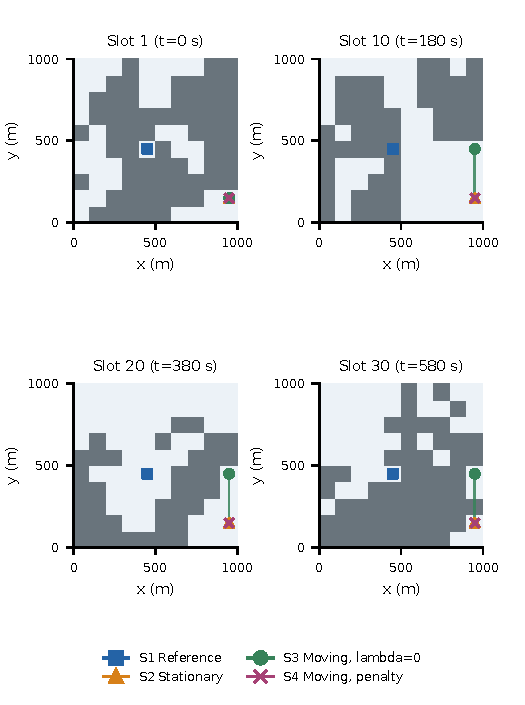
\includegraphics[width=\columnwidth]{figures/figure_1_single.pdf}
\caption{Binary cloud snapshots and MB UAV paths for the preregistered default realization 0. Dark cells are fully blocked links, indexed by UAV position; they are not geometric cloud footprints.}\label{fig:binary_1}\end{figure}

\begin{figure}[t]\centering
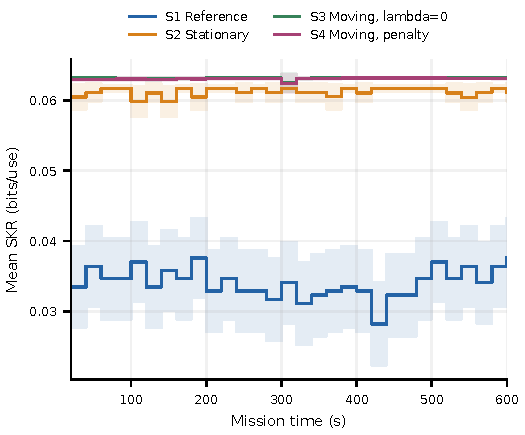
\includegraphics[width=\columnwidth]{figures/figure_2_single.pdf}
\caption{Mean per-slot diagnostic SKR for MB policies over 100 independent missions; shaded bands are 95% Monte Carlo t intervals for the mean.}\label{fig:binary_2}\end{figure}

\begin{figure}[t]\centering
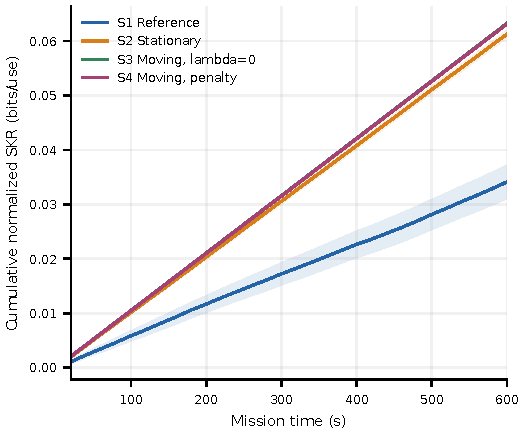
\includegraphics[width=\columnwidth]{figures/figure_3_single.pdf}
\caption{Mean cumulative normalized SKR sum(S)/N\_t. The endpoint equals mission-average SKR; it is not a finite-size key yield or a count of secret bits.}\label{fig:binary_3}\end{figure}

\begin{figure}[t]\centering
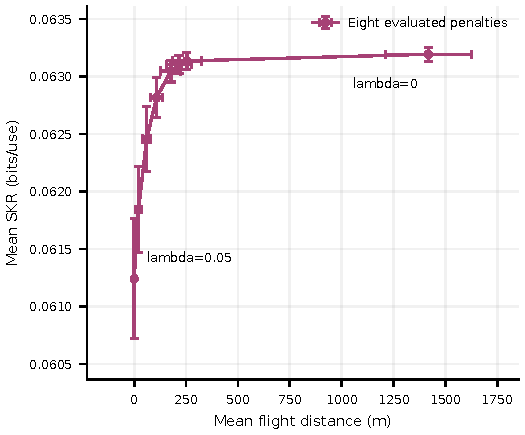
\includegraphics[width=\columnwidth]{figures/figure_4_single.pdf}
\caption{Mean MB SKR versus mean flight distance at the eight evaluated penalties. Lines connect evaluated points only and do not establish a continuous optimum.}\label{fig:binary_4}\end{figure}

\begin{figure}[t]\centering
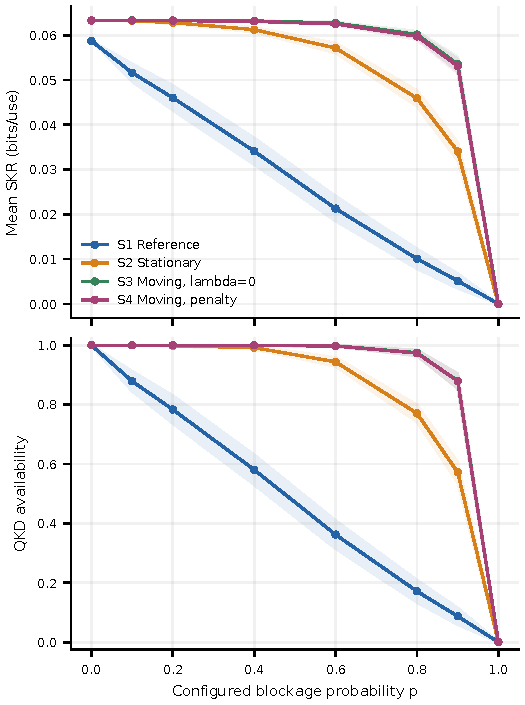
\includegraphics[width=\columnwidth]{figures/figure_5_single.pdf}
\caption{Average MB SKR and threshold availability versus configured blockage probability; all policies share each mission cloud matrix. Bands are mission-level Monte Carlo intervals.}\label{fig:binary_5}\end{figure}

\begin{figure}[t]\centering
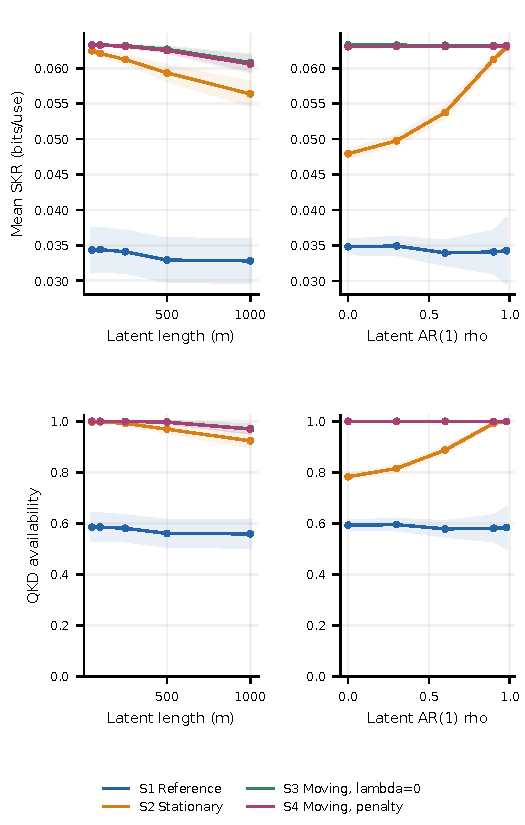
\includegraphics[width=\columnwidth]{figures/figure_6_single.pdf}
\caption{One-factor sensitivity to Gaussian latent spatial length and temporal AR(1) coefficient. Binary correlations differ from latent parameters; the other parameters retain their default values.}\label{fig:binary_6}\end{figure}

\begin{figure}[t]\centering
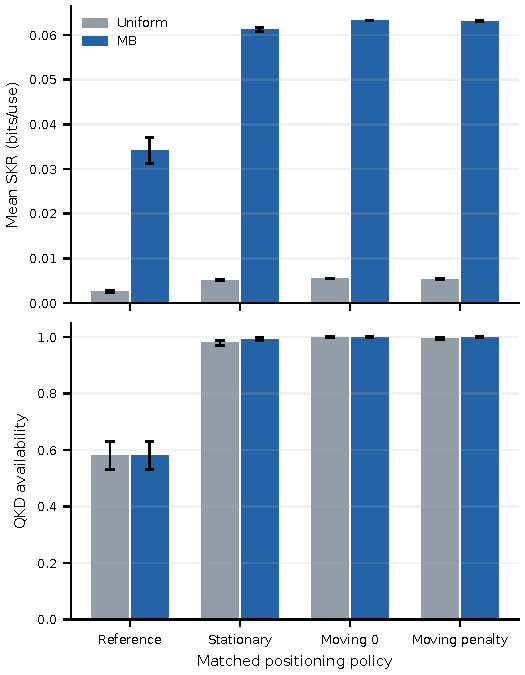
\includegraphics[width=\columnwidth]{figures/figure_7_single.pdf}
\caption{Paired MB and Uniform comparisons under the same four positioning policies and binary-cloud realizations. Each family optimizes its own exact finite source bank; selected energies can differ.}\label{fig:binary_7}\end{figure}
